%!TEX root = ../main.tex

\chapter{Design and Implementation}
This chapter follows the process of producing and optimising the artefact to fulfill the previously articulated objectives. The first section of the chapter follows the research on Google Safe Browsing's effective in detecting phishing websites. The accuracy target of the classifier implemented in this chapter is bounded by the results of the aforementioned case study.

The next section explores different machine learning algorithms and URL features, aiming to deliver satisfactory results in comparison with the threshold. After this, a number of features that could complement the machine learning solution are presented and assessed. Finally the classifier is brought together and assessed as a whole.

\section{Threshold definition}
Before attempting to improve the level of protection the most popular browsers offer, the system's effectiveness needs to be assessed. In doing so the behaviour of the user will be simulated using an browser automation framework in accessing confirmend phishing websites. The outcome of this serves as an accuracy threshold for the proposed artefact.

The first step of the process is data aquisition. A list of URLs pointing to online phishing webpages, confirmed to be malicious by the PhishTank community is fetched from their archive. The first test is run on the data available on the 1st on April. Testing a total number of 9345 phishing URLs, Google Safe-Broswing managed to achieve a total accuracy of 50.76\%.
The next test is run with the data published on the 7th of April. This time Google Safe-Browsing performed slightly worse reporting an accuracy of 48.32\% on the 8164 phishing URLs. Running the same test on the data aquired on the 1st of April shows a significant drop in accuracy, reporting an accuracy of 40.28\% on a number of 9359 URLs.

Upon a surface level inspection it is noticeable that given it's popularity in usage, Google Safe-Browsing influences the lifetime of a portion of phishing URLs. It is probable that attackers adapt to the situation and remove phishing webpages detected, or serve them through different URLs. Moving a webpage from one domain to another is not resource expensive and allows the attackers to dodge the browser's anti-phishing detection system.

Finally, the threshold is set to be the highest accuracy recorded across the two tests of 50.76\%.

\section{List based module}
It is safe to assume that most of web browsing activity takes place across a limited set of domains. This is reflected in different rankings of most popular domains. Because these are known to be benign, there is no reasong for wasting resources on the classification process. Because of this, a list based module is included in the phishing detection system.
The white-list included is comprised of the domains ranking published by \cite{MAJESTIC_MILLION}.

\section{Machine learning module}
As the current literature shows, there is a breadth of approaches in detection an prevention of phishing attacks. However, an emergent pattern in effective anti-phishing detection systems is the use of machine learning. A well trained and calibrated module of this kind increases the performance and robustness of the proposed artefact. Besides this, it offers the capability of dealing with newly registered phishing domains and URLs without further training.

\subsection{Experimentation details}
The first step in building this module is the selection of machine learning algroithms. The set used is based on the emergent pattern of algorithms used in the Background Study (\ref{chap:bgStudy}) and is composed of Naive Bayes, Decision Tree, Random Forest, Support Vector Machine. In addition to these, the multilayered perceptron neural network is added with the purpose of experimentation.

The dataset used for feature extraction and training is composed of 100,000 records. These are split in 40,000 benign URLs and 60,000 phishing.

\subsection{Features exploration}
The features extracted from given URLs are the basis for machine learning and classification. These should put emphasis on areas where the two classes of URLs differ. The aim of this subsection is to find correlations that best separate benign URLs from phishing ones. The process of feature selection is highly influenced by the dataset on which the exploration is done. Because this artefact competes with the most popular phishing detection system the chosen dataset is comprehensive in most aspects.

The feature selection process starts with URL length. The literature is clear on the discrepancy in average URL length between legitimate and phishing URLs. One example is illustrated in \cite{STACKED_ML_URL_HTML} (Figure \ref{fig:URL_LENGTH_DISTRIBUTION}), showing the distribution over a set of 50,000 URLs. Doing a URL length analisys (Table \ref{tab:URL_SIZE_ANALISYS}) on the dataset used in training the artefact, there is an obvious correlation between maliciousness and URL length.

\begin{figure}[t]
	\centering
	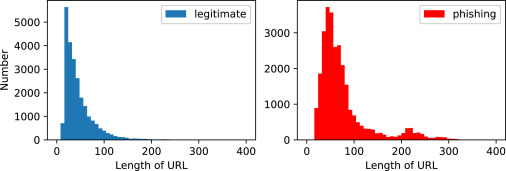
\includegraphics[width=0.9\textwidth]{url_length_50k.jpg}
	\caption{URL length distribution over a dataset of 50,000 records}
	\label{fig:URL_LENGTH_DISTRIBUTION}
\end{figure}

\begin{singlespace}
	\small
	\begin{center}
		\label{tab:URL_SIZE_ANALISYS}
		\begin{tabular}{ | m{8em} | m{13em} | m{8.5em} | m{2.3em} | m{5em} | }
			\hline
			                         & \textbf{benign} & \textbf{Phishing} \\
			\hline
			\textbf{Average}         & 57.81           & 77.54             \\
			\hline
			\textbf{Median}          & 52              & 52                \\
			\hline
			\textbf{90th percentile} & 90              & 147               \\
			\hline
			\textbf{95th percentile} & 107             & 220               \\
			\hline
			\textbf{99th percentile} & 141             & 321               \\
			\hline
		\end{tabular}
		\captionsetup{type=table}\caption{A comparison of existing solutions \citep{INTELLIGENT_PHISHING_ANFIS}}
	\end{center}
\end{singlespace}


The second feature selected is the protocol used. There is a case to be made agains using protocol as a feature due to its rise is usage shown in (). However, although TLS adoption is growing, serving a website through HTTPS requires technical knowledge and a certain amount of effort. Besides this, the low average lifespan of a phishing webpage could help the average attacker decide against using it. Based on these factors it is safe to assume that the number of phishing websites using TLS will not exceed 85\%.

Doing protocol analisys on the dataset shows that the lack of TLS usage and maliciousness are highly correlated.

The third feature selected is the number of numerical character in the domain and subdomain. The choice comes from the fact that it is highly uncommon for benign domains and subdomains to contain any numerical characters. This is confirmed by the analysis of the distribution of numerical characters throughout the dataset.

The fourth feature is the number of '@' and '~' characters. The reasoning behind this is that, like numerical characters, it is uncommon for an URL to contain any '~' characters. It is an outdated practice of accessing a user's folder appending their name after the '~' character.
The '@' is especially dangerous as it produces unexpected behaviour in the browser. It could either redirect to an email address using the default mail client or get the browser to ignore every character on it's rigth side.

The analysis of the dataset shows that although they do not occur as often, these characters are still indicative of malicious activity and can improve decision-making in the reduced number of cases it is present.


The fifth feature is the presence of a network location in the URL. Given the popularity of storage and hosting services today and the existence of many open redirect vulnerabilities, some phishing URLs hide their real domain behind the trusted domain of another company. This feature flags up the presence of such practice by checking if the number of dots in the path of the URL exceeds one.

The sixth feature chosen is the number of hyphens. Although it could be, this metric is not included as an indicator of maliciousness on it's own, but rather as a support metric to aid in decision making when considering the other features as well. If there is no domain present in the path portion of the URL, the hyphen count is determined based on the network location only, otherwise for the whole URL. This is done to cover cases such as "target-brand.example.com" and "storage.service.com/website/target-brand.example.com/"
In the case of the used dataset, there is no obvious correlation between number of hyphens and maliciousness

The seventh feature selected is the number of subdomains components. Most of benign URLs either use "www" as subodmain, or another arbitrary string of characters. But the thing they have in common is that they use only one subdomain component. Phishing URLs however, may use a multi-component subdomain to create the illusion of the target brand. Based on this reasoning, this feature will flag any URL whose subdomain components count exceeds two. With this configuration, the feature shows a slight correlation with the benign URLs

The eighth, nineth and tenth features flag the presence of sensitive vocabulary in the URL. \cite{10.1145/1314389.1314391} in the study of phishing url obfuscation techniques uncovered the correlation of a set of words with malicious intent. The study has been done in 2007, so in order to maximize the efficiency of the set of sensitive words, they need to be extracted from an updated set.

The word frequency count is performed on a coroboration of multiple phishtank(REF?) lists of valid phishes. These are split in the format of <subdomain>.<domain>/<path>?<query> and further probabilistically split concatenated words using natural language processing (NLP) based on English Wikipedia unigram frequencies.

Experimentation with the most frequent words extracted shows that the query section of the URL has the same key words as in benign URL, thus being prone to causing numerous false positives. Because of this, the final lists of sensitive words used are for the subdomain, domain and path section.

To further enhance the potential of this feature, the path and query sections of the URLs are searched for popular domains. Because it is a common practice in phishing URLs to use the target domain or brand in the path under the form of "www.example.com/brand/signin.html", if there is no sensitive word found in path, the first 2500 domains are searched throughout the path and query portions.

The last two features are based on the similarity between URL's domain and subdomain, and the top N benign domains. This feature directly targets the practice of brand obfuscation and the illusion of accessing a trusted domain.
Phishing URLs use an array of techniques to create this illusion. A comprehensive list of these techniques and mutations is presented in Table . All these permutations are done with the aim of tricking the viewer if they're not exercising a closer inspection.


Original example.com
Addition examplea.com
Bitsquatting azample.com
Homoglyph ēxãmple.com
Hyphenation exampl-e.com
Insertion examplme.com
Omission exaple.com
Repetition exxample.com
Replacement esample.com
Subdomain ex.ample.com
Transposition exapmle.com
Vowel-swap exomple.com
TLD inclusion examplecom.com

To flag such pattern feature 10 measures the Levenshtein distance between the target URL and the top 25,000 benign domains. The Levenshtein distance calculates the number of operations (additions, subtractions, insertions etc.) needed to be performed on one of the strings so that tey are identical. If the Levenshtein distance is lower or equal to five and different than zero, then the URL is flagged as suspicious.

The next feature does the same between all the components of the subdomain and the top 25,000 benign domains. In this case a distance lower than three will flag up the URL as suspicious

Illustrating the correlations between the URL labels (benign or malicious) and the selected set of features, shows how relevant these features are.

\begin{figure}[t]
	\centering
	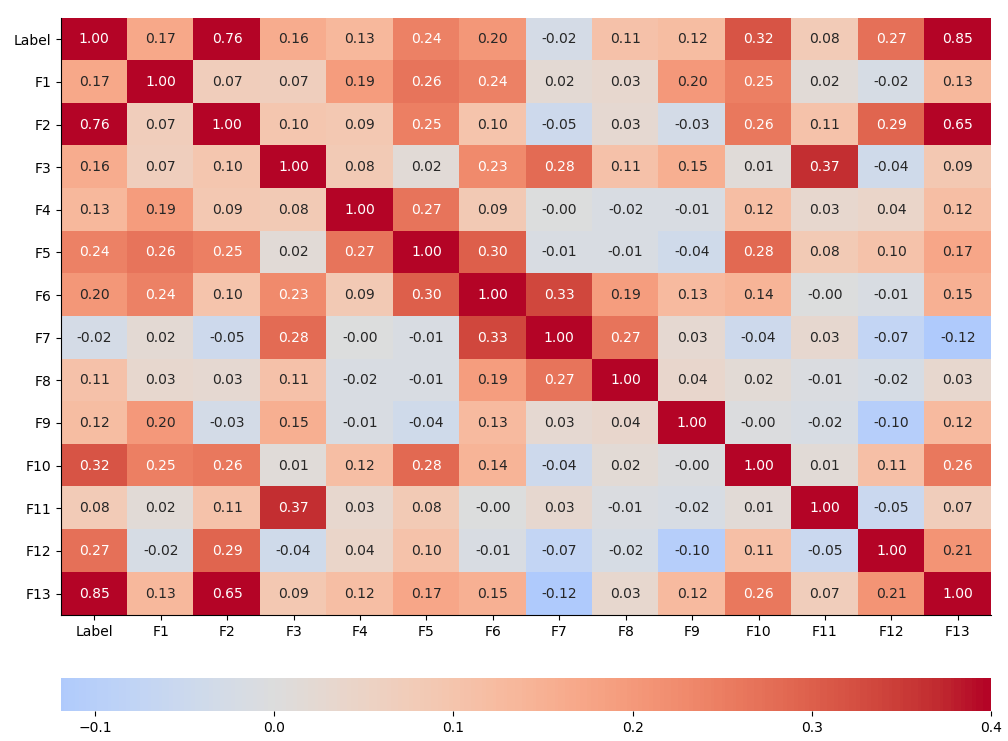
\includegraphics[width=1\textwidth]{feature_correlation.png}
	\caption{URL length distribution over a dataset of 50,000 records}
	\label{fig:FEATURE_CORRELATION}
\end{figure}

\section{Initial performance assessment}
This section follows the process of model training and initial performance assessment. Starting with training the first set of models shows the amount of effort put into feature extraction reflected in the results. Table \ref{tab:FIRST_TRAINED_MODELS} presents the F1 scores of the alorightms. F1-score is the metric used to generalize performance because its a composed measurement including precision and recall.

\begin{singlespace}
	\small
	\begin{center}
		\label{tab:FIRST_TRAINED_MODELS}
		\begin{tabular}{ | m{8em} | m{13em} | m{8.5em} | m{2.3em} | m{5em} | }
			\hline
			                                & \textbf{F1-score} \\
			\hline
			\textbf{Naive Bayes}            & 98.37             \\
			\hline
			\textbf{Decision Tree}          & 98.74             \\
			\hline
			\textbf{Random Forest}          & 98.86             \\
			\hline
			\textbf{Support Vector Machine} & 98.76             \\
			\hline
			\textbf{Multi-layer Perceptron} & 97.21             \\
			\hline
		\end{tabular}
		\captionsetup{type=table}\caption{A comparison of existing solutions \citep{INTELLIGENT_PHISHING_ANFIS}}
	\end{center}
\end{singlespace}

The algorithms show a major improvement in labeling the training data, surpassing the thershold by a large margin. However, the F-measure is not enough to get an insight into a model's performance. Two of the metrics that offer some transparency in performance are the Receiver Operating Characteristic (ROC) curve and Confusion matrix. The former illustrates how well a model is capable to distinguish between a phishing URL and a benign one while the latter shows the classification performance of the model.
An example of these measurements is presented in Figure \ref{fig:ROC_CM_EXAMPLE} for the Random Forest model. The maximum area under curve (AOC) shows that the model can easily distinguish between the two types of URLs. The confusion matrix shows that it is uncommon for the algorithm to mislabel URLs. In the example the random forest mislabeled 109 URLs out of 10,000.

\begin{figure}[t]
	\centering
	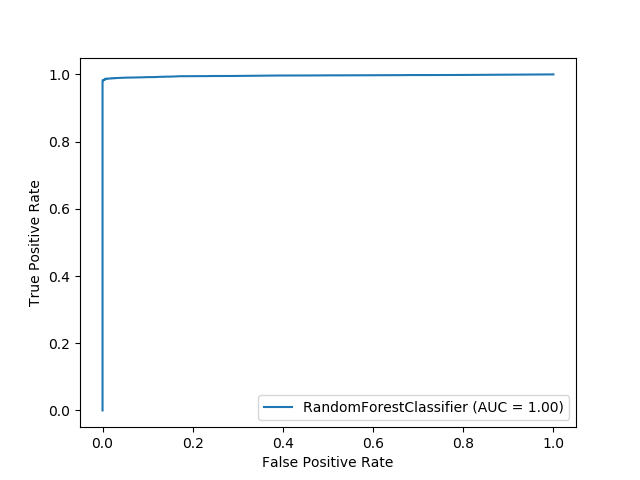
\includegraphics[width=0.49\textwidth]{rf_roc_example.png}
	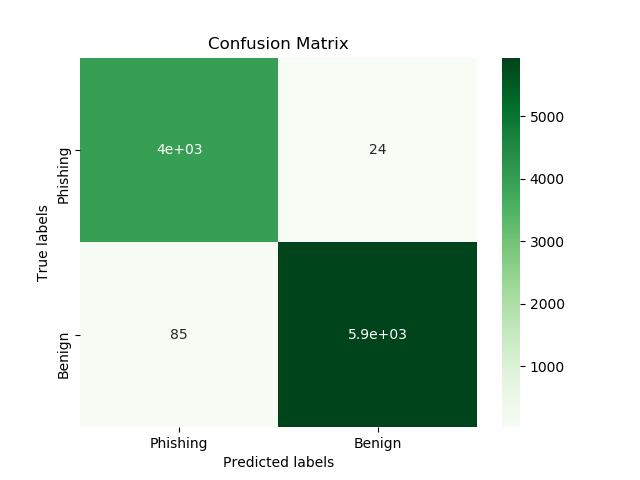
\includegraphics[width=0.49\textwidth]{rf_cm_example.png}
	\caption{URL length distribution over a dataset of 50,000 records}
	\label{fig:ROC_CM_EXAMPLE}
\end{figure}

An important factor in model selection and calibration is the amount of false positives produces. The literature states that the higher the delivery of false positives, the less the alerts are taken into consideration by the user. Because of this the final model needs to prioritise precision over recall and false negatives over false positives.

To test its performance in a realistic scenario, the models are set to deliver predictions on the remainder benign and phishing URLs of the 450,000 dataset. The results collected from the predictions over 305,737 benign URLs and 74,436 phishing urls are presented in Table (REF)


% NEEDS TO BE RERUN
\begin{singlespace}
	\small
	\begin{center}
		\label{tab:FIRST_TRAINED_MODELS}
		\begin{tabular}{ | m{8em} | m{13em} | m{8.5em} | m{2.3em} | m{5em} | }
			\hline
			                                & \textbf{Precision} &\textbf{Sensitivity} &\textbf{F1-score}& \textbf{Accuracy}  \\
			\hline
			\textbf{Naive Bayes}            & 89.86  & 99.28 & 94.34 &97.66        \\
			\hline
			\textbf{Decision Tree}          & 95.10 & 99.12 & 97.07 & 98.83        \\
			\hline
			\textbf{Random Forest}          & 94.71 & 88.17 & 96.89 & 98.75      \\
			\hline
			\textbf{Support Vector Machine} & 94.88 &99.16&96.97&98.78 \\
			\hline
			\textbf{Multi-layer Perceptron} & 19.57 & 100 & 32.74 & 19.57   \\
			\hline
		\end{tabular}
		\captionsetup{type=table}\caption{A comparison of existing solutions \citep{INTELLIGENT_PHISHING_ANFIS}}
	\end{center}
\end{singlespace}


The next dataset used to evauate model performance is composed of online and valid phishes from 1st of April. This way the models are tested on the same parameters Google safe browsing was.

\begin{singlespace}
	\small
	\begin{center}
		\label{tab:FIRST_TRAINED_MODELS}
		\begin{tabular}{ | m{8em} | m{13em} | m{8.5em} | m{2.3em} | m{5em} | }
			\hline
			                                & \textbf{Precision} &\textbf{Sensitivity} &\textbf{F1-score}& \textbf{Accuracy}  \\
			\hline
			\textbf{Naive Bayes}            & 1.00  & 83.33 & 90.91 &83.33        \\
			\hline
			\textbf{Decision Tree}          & 1.00 & 81.15 & 89.59 & 81.15        \\
			\hline
			\textbf{Random Forest}          & 1.00 & 82.11 & 90.17 & 82.11      \\
			\hline
			\textbf{Support Vector Machine} & 1.00 &78.91&88.21&78.91 \\
			\hline
			\textbf{Multi-layer Perceptron} & 1.00 & 82.69 & 90.52 & 82.69   \\
			\hline
		\end{tabular}
		\captionsetup{type=table}\caption{A comparison of existing solutions \citep{INTELLIGENT_PHISHING_ANFIS}}
	\end{center}
\end{singlespace}


\section{Performance improvement}
Given the results of the models presented in the previous section, the performance improvement shown in this section is not expected to be substantial.
The first step in improving the performance is removing features with a correlation to the label close to zero. The correlation matrix presented in Figure (REF) shows feature number seven as having the lowest correlation to the label. Removing the long subodmain feature reduces confusion in model training and offers a slight improvement in delivering accurate predictions. Figure \ref{fig:IMPROVED_FEATURE_CORRELATION} illustrates the correlation heatmap after removal.

\begin{figure}[t]
	\centering
	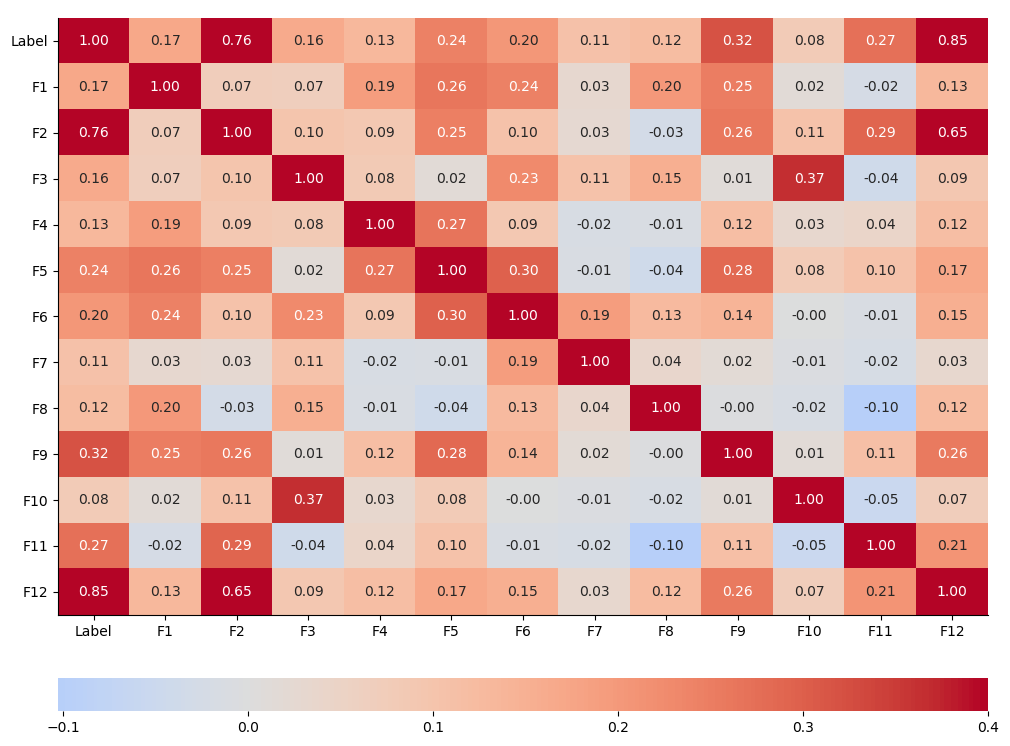
\includegraphics[width=1\textwidth]{improved_feature_correlation.png}
	\caption{URL length distribution over a dataset of 50,000 records}
	\label{fig:IMPROVED_FEATURE_CORRELATION}
\end{figure}

The second step is hyperparameter tuning. The process of hyperparameter tuning or optimisation consists of training the subject model with different values for it's parameters. By trying different permutations of values for these parameters the trained model delivers better or worse predictions and can be selected for further optimisation based on this.

Hyperparameter tuning is resource expensive. Because of this, the algorithms selected for optimisations are the ones that already deliver good and consistent results. These are the random forest, the support vector machine and the multi-layer perceptron classifiers.

%METHODOLOGY?
The calibration is done using GridSearchCV. GridSearchCV does and exhaustive search over specified parameters and selects the best performing model. 

Starting with the optimisation of the random forest classifier, the number of the n\_estimators is increased to raise the number of decision trees. By doing so the model delivers better predictions at the expense of both training an prediction time. Because of this the number of n\_estimators is set to a reasonable set of values comprised of 1600, 1800 and 2000. Next the max\_depth of each decision tree is set to be either 8,12 or 16. The last calibration is done on the max\_features parameter. This sets the number of maximum features provided to each tree and will be tested with the values of auto and sqrt.

The calibration of the SVM classifier is done by searching for the best performing C parameter. The C parameter influences the missclassification threshold of the model. With a greater C value, the classifier will chose a smaller-margin hyperplane rendering the model less prone to deliver wrong predictions. However, a bigger C value will increase the chance of overfitting. Having said that, the values of the C fed into the GridSearchCV are 10,100 and 1000.

Given the opaque nature of the training process of neural networks, the calibration of the multi-layer perceptron resembles more a hit-or-miss experimentation. Because of this, different models have been trained using most of the optimisation parameters that the MLP classifier takes as input.

\begin{singlespace}
	\small
	\begin{center}
		\label{tab:OPTIMISED_MODELS}
		\begin{tabular}{ | m{8em} | m{13em} | m{8.5em} | m{2.3em} | m{5em} | }
			\hline
			                                & \textbf{F1-score} & \textbf{F1-score (optimised)} & \textbf{Delta}\\ 
			\hline
			\textbf{Random Forest}          & 98.86  & 98.91  & 0.05         \\
			\hline
			\textbf{Support Vector Machine} & 98.76  &98.87   & 0.11       \\
			\hline
			\textbf{Multi-layer Perceptron} & 97.21   & 98.76  & 1.25        \\
			\hline
		\end{tabular}
		\captionsetup{type=table}\caption{A comparison of existing solutions \citep{INTELLIGENT_PHISHING_ANFIS}}
	\end{center}
\end{singlespace}

As expected, the results of the optimisation (Table \ref{tab:OPTIMISED_MODELS}) did not deliver a substantial improvement. This is partly because they already achieved impressive results. The optimisation has shown improvements in the confusion matrix and ROC curve as well. Figures (REF) show that the AUC has a maximum value while figures (REF) show that the low rate of false positives is prioritised over 




% ROC curve and Confusion matrixes plus discuss parameters and cross validation (here and in the methodology) 









%=========================================================================================================
% Skipped compiling instructions
\iffalse
	You should always start with an overview (Heading 2 style) to tell what this chapter is about and finish with a summary (Heading 2 style) to tell what has been covered in this chapter.

	The Design and Implementation chapter should explain the design technique chosen and justify why it is appropriate, depending on the development methodology.  Suitable diagram-techniques (e.g. UML, other drawings) should be used where appropriate. For the Implementation part, it should talk about the technical realisation of the concepts and ideas developed earlier. It is used to describe the system at a finer level of technical details, down to the code level. However, do not attempt to describe all the code in the system, and do not include large pieces of code in this section.

	You should highlight the pieces of code which are critical to the system or worth to be noted. For example, the creation and/or implementation of core algorithms that make the system functional or some methods/ways you have used which are non-standard or innovative in the system implementation. You should also mention any unforeseen problems you encountered when implementing the system and how and to what extend you overcame them.

	Appropriate testing must also be included in this section







	The starting set in feature selection is based on the work of \cite{SVM_SIMILARITY_INDEX}. The choice is based on the solution's use of similarity indexes in model training. These similarity indexes are highly relevant as most phishing URLs try to decieve the victims by including different variations of the target brand or domain. Besides this, the model reports an accuracy of 95\% far exceeding the set threshold.

	The first feature selected is URL length. The literature is clear on the discrepancy in average URL length between legitimate and phishing URLs. One example is illustrated in \cite{STACKED_ML_URL_HTML} (Figure \ref{fig:URL_LENGTH_DISTRIBUTION}), showing the distribution over a set of 50,000 URLs.

	\begin{figure}[t]
		\centering
		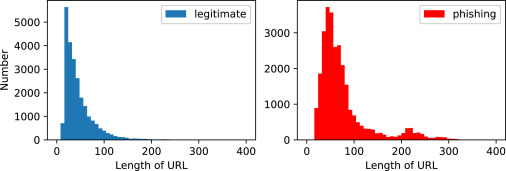
\includegraphics[width=0.9\textwidth]{url_length_50k.jpg}
		\caption{URL length distribution over a dataset of 50,000 records}
		\label{fig:URL_LENGTH_DISTRIBUTION}
	\end{figure}

	The second feature chosen is the number of hyphens. It is common for phishing URLs to use such characters to deceive the victim by chaining the target brand using hyphens (e.g. www.example-secure-bank.com).

	The third feature is the number of dots. This is used in a simmilar manner as hyphens are, only it allows for using subdomains to create the illusion of the legitimate page (e.g. www.example.secure.bank.com)

	The fourth feature is the number of numerical characters present in the domain. This is included because it is uncommon for legitimate domains to contain any numerical characters.

	The fifth is the presence of an IP address in the URL. Although substantially less prevalent in current phishing attacks, it still happens that some of the phishing URLs are not addressed by domain name, but by IP address. This is a solid indicator that the URL may point to a phishing webpage.

	The last feature is the Hamming distance between the URL to be classified and a top N benign domains. Similarity indexes like the Hamming distance calculate the distance of two pieces of data, in this case the distance between two strings of characters. It does so through a mathematical formula which outputs 0 or 100 on identical strings depending on implementation. For the first test the algorithm is trained with the maximum hamming distance between the input URL and top 1000 benign domains from the \cite{MAJESTIC_MILLION} dataset.

	\begin{figure}
		\centering
		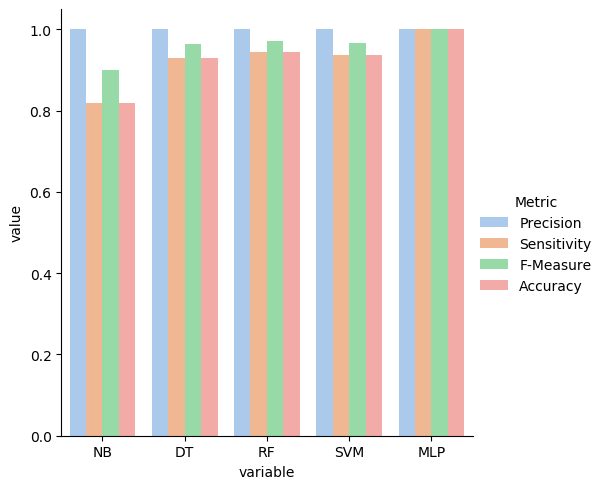
\includegraphics[width=0.49\textwidth]{hamming5k_on_phishtank_0401.png}
		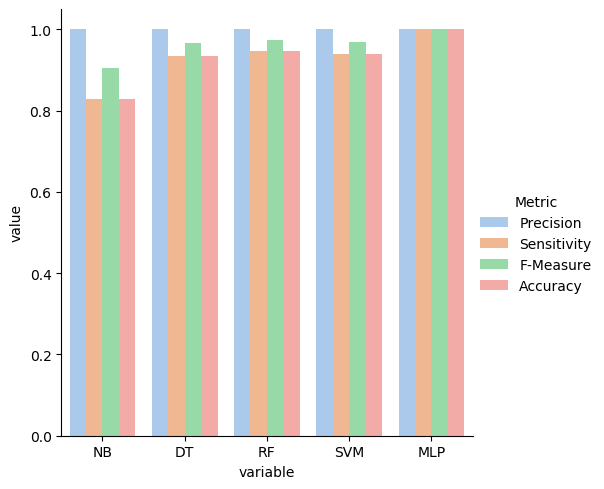
\includegraphics[width=0.49\textwidth]{hamming5k_on_phishtank_0405.png}
		\caption{URL length distribution over a dataset of 50,000 records}
		\label{fig:HAMMING_ON_PHISHTANK}
	\end{figure}

	The results of this feature compilation are far exceeding Google Safe-Browsing's accuracy. However when the models are evaluated on a dataset that includes benign URLs the metrics show a significant drop in every aspect exept sensitivity. Figure \ref{fig:HAMMING_ON_MIXED} illustrates the bias of the model towards classifying URLs as malicious on a 5,000 records dataset (left side) and a 25,000 dataset (right side). Both the datasets are composed of half benign urls, half malicious.

	\begin{figure}[b]
		\centering
		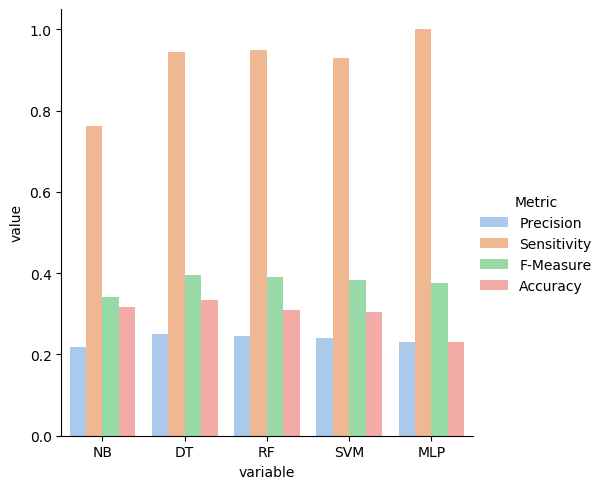
\includegraphics[width=0.49\textwidth]{hamming5k_on_mixed.png}	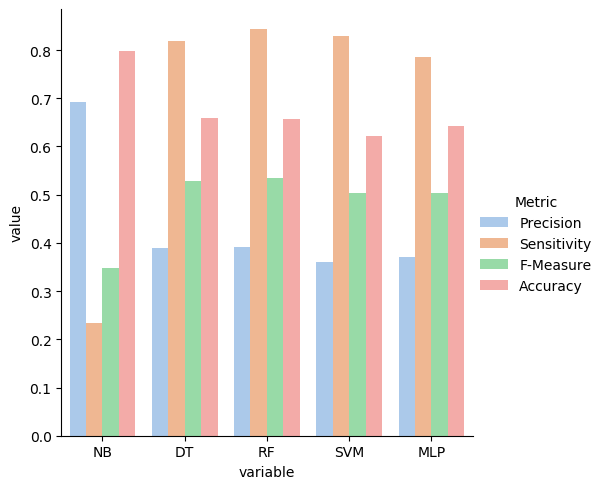
\includegraphics[width=0.49\textwidth]{hamming25k_on_mixed.png}
		\caption{URL length distribution over a dataset of 50,000 records}
		\label{fig:HAMMING_ON_MIXED}
	\end{figure}

	These results differ from what is reported by \cite{SVM_SIMILARITY_INDEX} because the models are trained on different datasets. Given the circumstances, the next step is improving the accuracy and lower the sensitivity by tweaking the features. The aim of this process is to increase the information known through features, helping the model in achieving better classifications.

	Firstly, the number of hypens will be expanded to the number of '@', '-' and '~' symbols. The '@' sign is a particularly suspicious, as browsers ignore the characters placed on it's right side when parsing the URL. The number of numerical characters is set not only with the domain as input, but with both domain and subdomain. The reasoning being that it is equally uncommon to have subdomains containing digits.

	\begin{figure}[t]
		\centering
		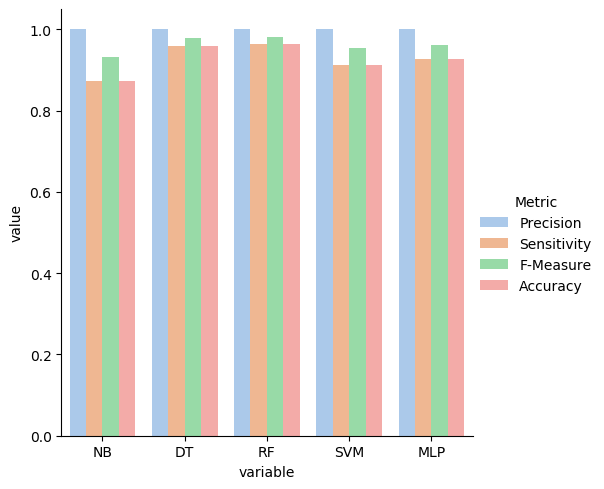
\includegraphics[width=0.49\textwidth]{levenshtein5k_on_phishtank_0401.png}	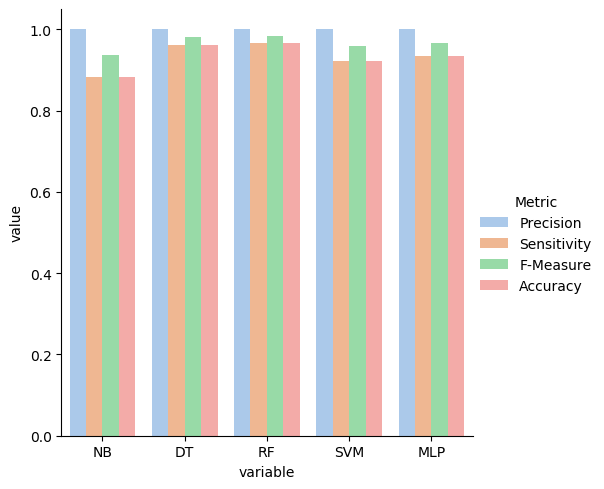
\includegraphics[width=0.49\textwidth]{levenshtein5k_on_phishtank_0405.png}
		\caption{URL length distribution over a dataset of 50,000 records}
		\label{fig:HAMMING_ON_MIXED}
	\end{figure}

	The Hamming distance is designed to calculate the distance between two strings of equal length. Because of this, when computing the Hamming distance between two domains one of them needs to be padded. Because of this the Hamming distance is swapped for the Levenshtein distance. There is no performance loss expected as \cite{SVM_SIMILARITY_INDEX} reports similar results in both similarity indexes. Furthermore, these distances will not only be calculated between the malicious domain and benign list of domains, but between the list of benign domains and both malicious subdomain strings separated by periods and the domain. The aim of this addition is to increase model's awareness regarding domains such as "www.bank.secure.brand.com".

	Illustrating the correlations between the URL labels (benign or malicious) and the selected set of features, shows how relevant these features are.

	\begin{figure}[b]
		\centering
		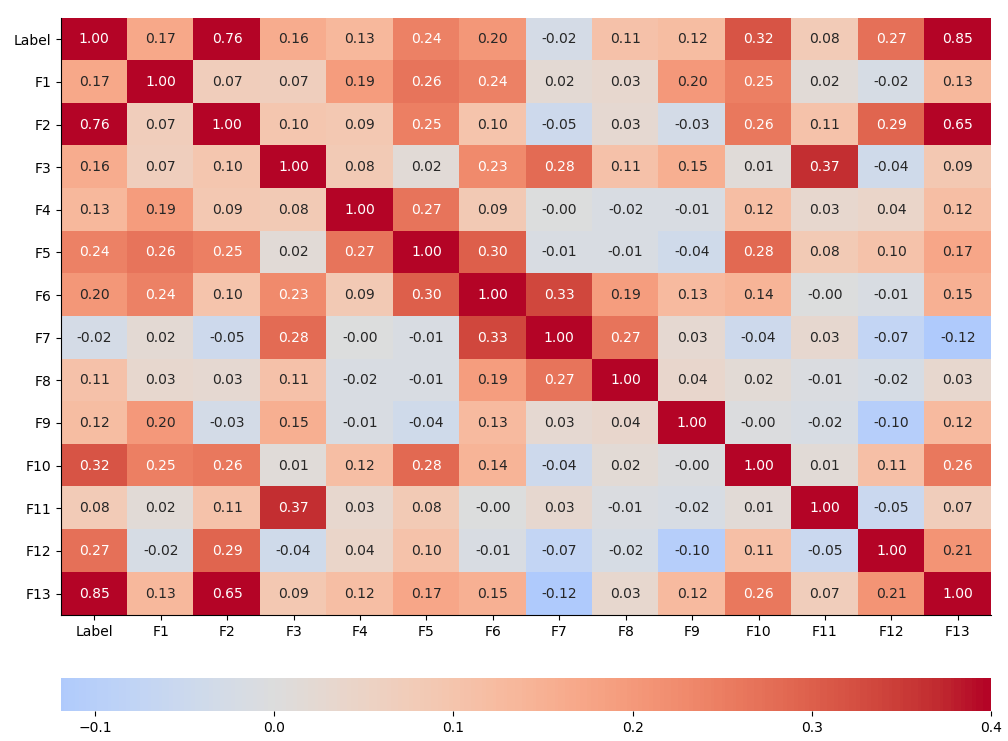
\includegraphics[width=0.49\textwidth]{feature_correlation.png}
		\caption{URL length distribution over a dataset of 50,000 records}
		\label{fig:FEATURE_CORRELATION}
	\end{figure}





	1. Dont forget to discuss dataset exploration
	4. Mention that the aim is for this artefact tot be lightweight and show how much plain static URL analysis can achieve
	5. Revisit the number of phishing attacks

\fi